\documentclass[]{standalone}
\usepackage[T1]{fontenc}
\usepackage{tikz}
\usepackage{amsmath, amsfonts}
\usepackage{xintexpr}
\usepackage{comment}
\usepackage{ifthen}
\usetikzlibrary{arrows, shapes.geometric, calc, positioning, decorations.pathreplacing, patterns.meta}

\makeatletter
\def\input@path{{./includes/}{./includes/ut/diags/}}
\makeatother

\definecolor{malachite}{rgb}{0.04, 0.85, 0.32}
\definecolor{mikadoyellow}{rgb}{1.0, 0.77, 0.05}

\begin{document}%
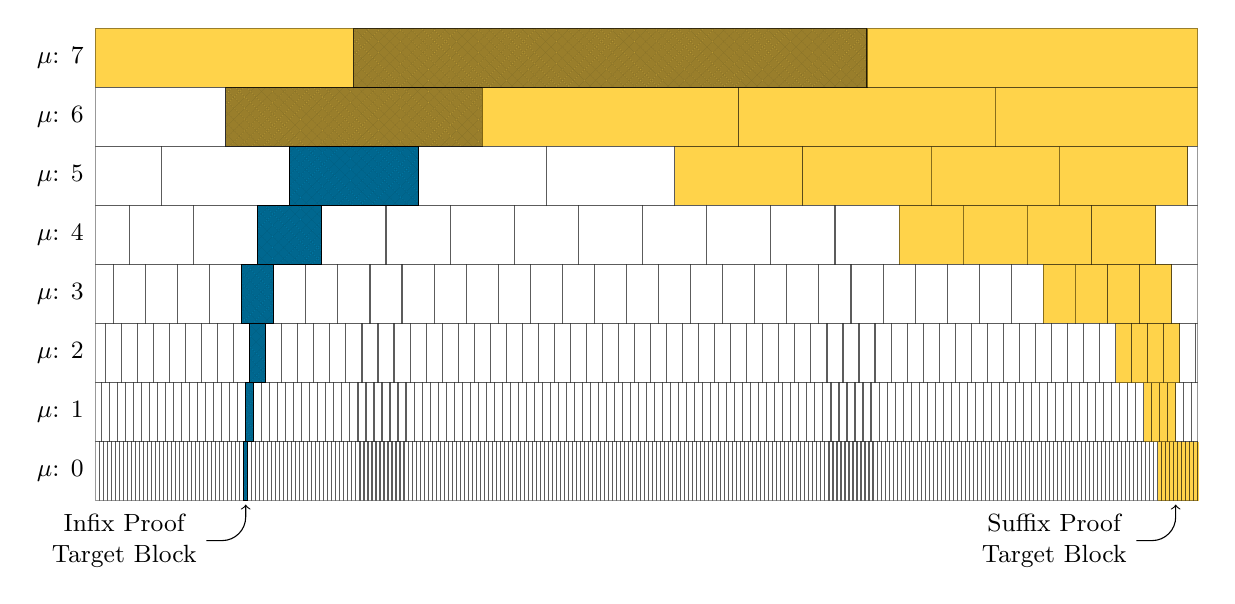
\begin{tikzpicture}[node distance=0.1cm]%
    \def\maxMu{7}
    \pgfmathtruncatemacro{\hlSuperMu}{\maxMu - 2}
    \pgfmathtruncatemacro{\nBlocks}{2^(\maxMu+1) + 19}
    \pgfmathtruncatemacro{\proofAnchor}{\nBlocks-6}
    \pgfmathtruncatemacro{\focusBlock}{37}
    \def\pgwidth{140}  % mm
    \pgfmathsetmacro\blockW{\pgwidth / \nBlocks}
    \pgfmathsetmacro\offs{\blockW/2}
    \xdef\blockH{7.5}
    \foreach \m in {0,...,\maxMu}{
        \pgfmathtruncatemacro{\nBlocksAt}{ceil(\nBlocks / (2^\m))}
        \pgfmathtruncatemacro{\twoTTMu}{2^\m}
        \pgfmathsetmacro\thisBWidth{\blockW * 2^\m}
        \pgfmathtruncatemacro\nextM{\m + 1}
        \foreach \x in {0,...,\nBlocksAt}{
            \pgfmathtruncatemacro\nextX{\x + \twoTTMu}
            \pgfmathsetmacro\xStart{max(-\offs, \x * \thisBWidth - 0.5*\thisBWidth)}
            \pgfmathsetmacro\xEnd{min(\x * \thisBWidth + 0.5*\thisBWidth, \pgwidth - \offs)}
            \pgfmathtruncatemacro\isOkay{\xStart < \xEnd}
            \ifnum 1=\isOkay
                % block numbers to focus on
                \pgfmathtruncatemacro\lower{(2*\x-5)*2^(\m-1)}
                \pgfmathtruncatemacro\upper{(2*\x+5)*2^(\m-1)}
                \pgfmathtruncatemacro\upperHead{(2*\x+8)*2^(\m-1)}

                \pgfmathtruncatemacro\myHeight{\x*2^\m}
                \pgfmathtruncatemacro\prevSBH{(\x-1)*2^\m}
                \pgfmathtruncatemacro\nextSBH{(\x+1)*2^\m}

                \pgfmathtruncatemacro\isFocusBlock{(\prevSBH < \focusBlock && \myHeight >= \focusBlock)}
                \pgfmathtruncatemacro{\isMainProof}{\proofAnchor <= \upperHead && (\myHeight <= \proofAnchor || (\myHeight > \proofAnchor && \m == 0))}
                \def\blockStyle{}
                % check if this block will be used as part of the NIPoPoW
                \pgfmathtruncatemacro{\isSuper}{0 && mod(\x, 2^(\hlSuperMu-\m+1)) == 0}
                \pgfmathtruncatemacro{\setBlockStyle}{\isSuper || \isFocusBlock || \isMainProof}

                \def\mpStyle{}
                \def\focusStyle{}

                \ifnum 1=\isMainProof
                    \def\mpStyle{fill=mikadoyellow}
                \fi

                \ifnum 1=\isFocusBlock
                    \def\focusStyle{pattern color=black, pattern={Hatch[angle=-45, distance=1mm, line width=1mm]}}

                    \ifnum 0=\isMainProof
                        \draw [fill=cyan] (\xStart mm, \m*\blockH mm) rectangle (\xEnd mm, \nextM*\blockH mm);
                    \else
                        \def\mpStyle{}
                        \draw [fill=mikadoyellow, opacity=.4, fill opacity=.75] (\xStart mm, \m*\blockH mm) rectangle (\xEnd mm, \nextM*\blockH mm);
                    \fi
                \fi
                \draw [opacity=.4, fill opacity=.75, style/.expanded=\mpStyle, style/.expanded=\focusStyle] (\xStart mm, \m*\blockH mm) rectangle node (b-\m-\x) {} (\xEnd mm, \nextM*\blockH mm);

                \pgfmathtruncatemacro{\proofAnchor}{(\m == 0) && (\x == \proofAnchor)}

                % \ifnum 1=\isTargetBlock
                % \fi
            \fi
        }
        \pgfmathsetmacro{\muLabelH}{(\m+0.5)*\blockH}
        \node [anchor=east] at (-0.1*\blockW, \muLabelH mm) {\small $\mu$: \m};
    }
    % \node [draw] at (7.5cm, 8cm) {test};
    \node (tgLabel) [anchor=north east, align=center, xshift=-5mm, yshift=-3mm, font=\small] at (b-0-\focusBlock.south) { Infix Proof \\ Target Block };
    \draw [->, rounded corners=3mm] (tgLabel.east) -| ([yshift=-3mm]b-0-\focusBlock.south);
    \node (paLabel) [anchor=north east, align=center, xshift=-5mm, yshift=-3mm, font=\small] at (b-0-\proofAnchor.south) { Suffix Proof \\ Target Block };
    \draw [->, rounded corners=3mm] (paLabel.east) -| ([yshift=-3mm]b-0-\proofAnchor.south);
\end{tikzpicture}%
\end{document}
